\documentclass[../main.tex]{subfiles}

%FOR SCRIBES: Please change the next three lines to reflect the correct
%FOR SCRIBES: lecture number, name, and date.
\newcommand{\counter}{0}
\newcommand{\lecturenumber}{{2022/03/22}}
\newcommand{\scribename}{{Hari Krishnan CK}}
\newcommand{\lecturedate}{15 April 2021} 

\begin{document}
\chapter{Lecture 2022/03/22} 

		%{	\color{blue}   \textbf{Edit the parts in blue and remove this part}}
		\begin{center}
			\framebox{\parbox{6.5in}{
					{\bf{ELL888 Indian Institute of Technology Delhi} }\\ 
					{\bf  {\color{blue} Lecture \; {Kernel methods, SVM regression: An overview}}}
					\\
					{Scribed by: {\color{blue}\textit{Hari Krishnan CK}}
					\\ Instructors: Prof.Sandeep Kumar and Prof.Jayadeva}
			}}
			\ \\
		\end{center}
%		\noindent{\bf Note}: {LaTeX template courtesy of UC Berkeley EECS dept.}
		
		\noindent {\bf Disclaimer}: {These notes have not been subjected to the
			usual scrutiny reserved for formal publications.  They may be distributed
			outside this class only with the permission of the Course Coordinator.}
		\vspace*{4mm}
		\setcounter{section}{\counter}
		%FOR SCRIBES: ---------- Begin Scribing Here ------------------------

\newpage

%%%%%%%%%%%%%%%%%%%%%%%PAGE-1%%%%%%%%%%%%%%%%%%%%%%
\section{Recap of previous lectures and basics}
In the previous lectures we have gone through the definition of Hilbert space and RKHS. We had also gone through the formulation of SVM and MCM for the linear case. We will go over them briefly below as recap.
    \subsection{Hilbert space}
    A vector space equipped with an inner product is defined as an inner product space.An inner product induces the notion of norm which is defined as $\|x\|=\langle x, x\rangle^{\frac{1}{2}}$. Norm introduces the notion of distance between points $ d(x,y)=\langle x, y\rangle^{\frac{1}{2}}$.
    \newline
    A sequence in a metric space is termed as Cauchy is there exists an N for all $\zeta$>0 such that $$d\left(x_{n}, x_{m}\right)<\zeta \quad \forall m, n \geq N$$.The space where all Cauchy sequences are convergent is called a complete space.A complete inner product space is called as a Hilbert space.So in short an inner product space where all Cauchy sequences converge is known as a Hilbert space.
    \subsection{Kernels}
Given an abstract space $\mathcal{X}$ a function which maps $\kappa: \mathcal{X} \times \mathcal{X} \mapsto \mathbb{R}$ is called a kernel function. Kernel functions are used to quantify the similarity between two points $\mathbf{x}$ and $\mathbf{x}^{\prime}$ in $\mathcal{X}$.
A kernel function typically satisfies the following two properties (but this is not required for all kernel methods). 
$$
\begin{aligned}
&\text { (symmetric) } \forall \mathbf{x}, \mathbf{x}^{\prime} \in \mathcal{X}, \kappa\left(\mathbf{x}, \mathbf{x}^{\prime}\right)=\kappa\left(\mathbf{x}^{\prime}, \mathbf{x}\right) \\
&\text { (non-negative) } \forall \mathbf{x}, \mathbf{x}^{\prime} \in \mathcal{X}, \kappa\left(\mathbf{x}, \mathbf{x}^{\prime}\right) \geq 0
\end{aligned}
$$

    \subsection{SVM for linearly separable case}
We will briefly go over the optimisation problem for SVM in linear case.The main idea is to maximise the margin between the two classes which is given by $\frac{2}{\|w\|}$.Instead of maximising the margin we solve a minimisation problem which tries to maximise margin and also tries to correctly classify samples.
$$\begin{aligned}
\min \quad & \frac{1}{2} w^{T} w \\
\text { subject to } \quad & y_{i}\left[w^{T} x_{i}+b\right] \geq 1, i=1, \ldots, l .
\end{aligned}$$
The corresponding dual is obtained by writing the Lagrangian and KKT conditions. The dual optimisation problem is given by $$
\max \quad q(\mu)=\sum_{i=1}^{l} \mu_{i}-\frac{1}{2} \sum_{i, j=1}^{l} \mu_{i} \mu_{j} y_{i} y_{j} x_{i}^{T} x_{j}
$$
subject to $\quad \mu_{i} \geq 0, \forall i$
$$
\sum_{i=1}^{l} \mu_{i} y_{i}=0
$$
For a convex optimisation problem both primal and dual will give the optimum solution.

\section{Introduction to Kernels}
    \subsection{Kernel function and Kernel matrices}
Given an abstract space $\mathcal{X}$ a function which maps $\kappa: \mathcal{X} \times \mathcal{X} \mapsto \mathbb{R}$ is called a kernel function. Kernel functions are used to quantify the similarity between two points $\mathbf{x}$ and $\mathbf{x}^{\prime}$ in $\mathcal{X}$.
A kernel function typically satisfies the following two properties (but this is not required for all kernel methods). 
$$
\begin{aligned}
&\text { (symmetric) } \forall \mathbf{x}, \mathbf{x}^{\prime} \in \mathcal{X}, \kappa\left(\mathbf{x}, \mathbf{x}^{\prime}\right)=\kappa\left(\mathbf{x}^{\prime}, \mathbf{x}\right) \\
&\text { (non-negative) } \forall \mathbf{x}, \mathbf{x}^{\prime} \in \mathcal{X}, \kappa\left(\mathbf{x}, \mathbf{x}^{\prime}\right) \geq 0
\end{aligned}
$$
Suppose we are given a kernel function $\kappa$, and elements $x_{1}, x_{2}, \ldots, x_{m} \in \chi_{\text {, }}$ $m \times m$ matrix $K$ such that
$$
K_{i j}=\kappa\left(x_{i}, x_{j}\right)=K_{j i}
$$
then the matrix $K$ is called as gram matrix of the kernel function $\kappa$ w.r.t the $m$ elements of the domain set $\chi$.
A Positive Definite Kernel is the kernel function which satisfies the equation given below:
$$
\sum_{i=1}^{m} \sum_{j=1}^{m} \alpha_{i} \alpha_{j} k\left(x_{i}, x_{j}\right) \geq 0
$$
Where, $\alpha_{t} \in \mathbb{R}$.We will be discussing more on Positive Definite Kernels while discussing Mercer's theorem.
    
    \subsection{Cover's Theorem}
    Cover's theorem is a fundamental theorem on which the basis of kernel based methods lie. The theorem states that if we have a data which is not linearly separable then we should be able to transform the data to a sufficiently high dimension via a non-linear transform where it is linearly separable.
    \newline
    An example of the data which is not linearly separable in 2D but is separable in 3D is given below. Note that we don't need to transform the data to very high dimensions always to get linearly separability, it could be possible with just increasing one dimension via a non-linear map. The idea is illustrated in the image given below
    \begin{figure}[htp]
    \centering
    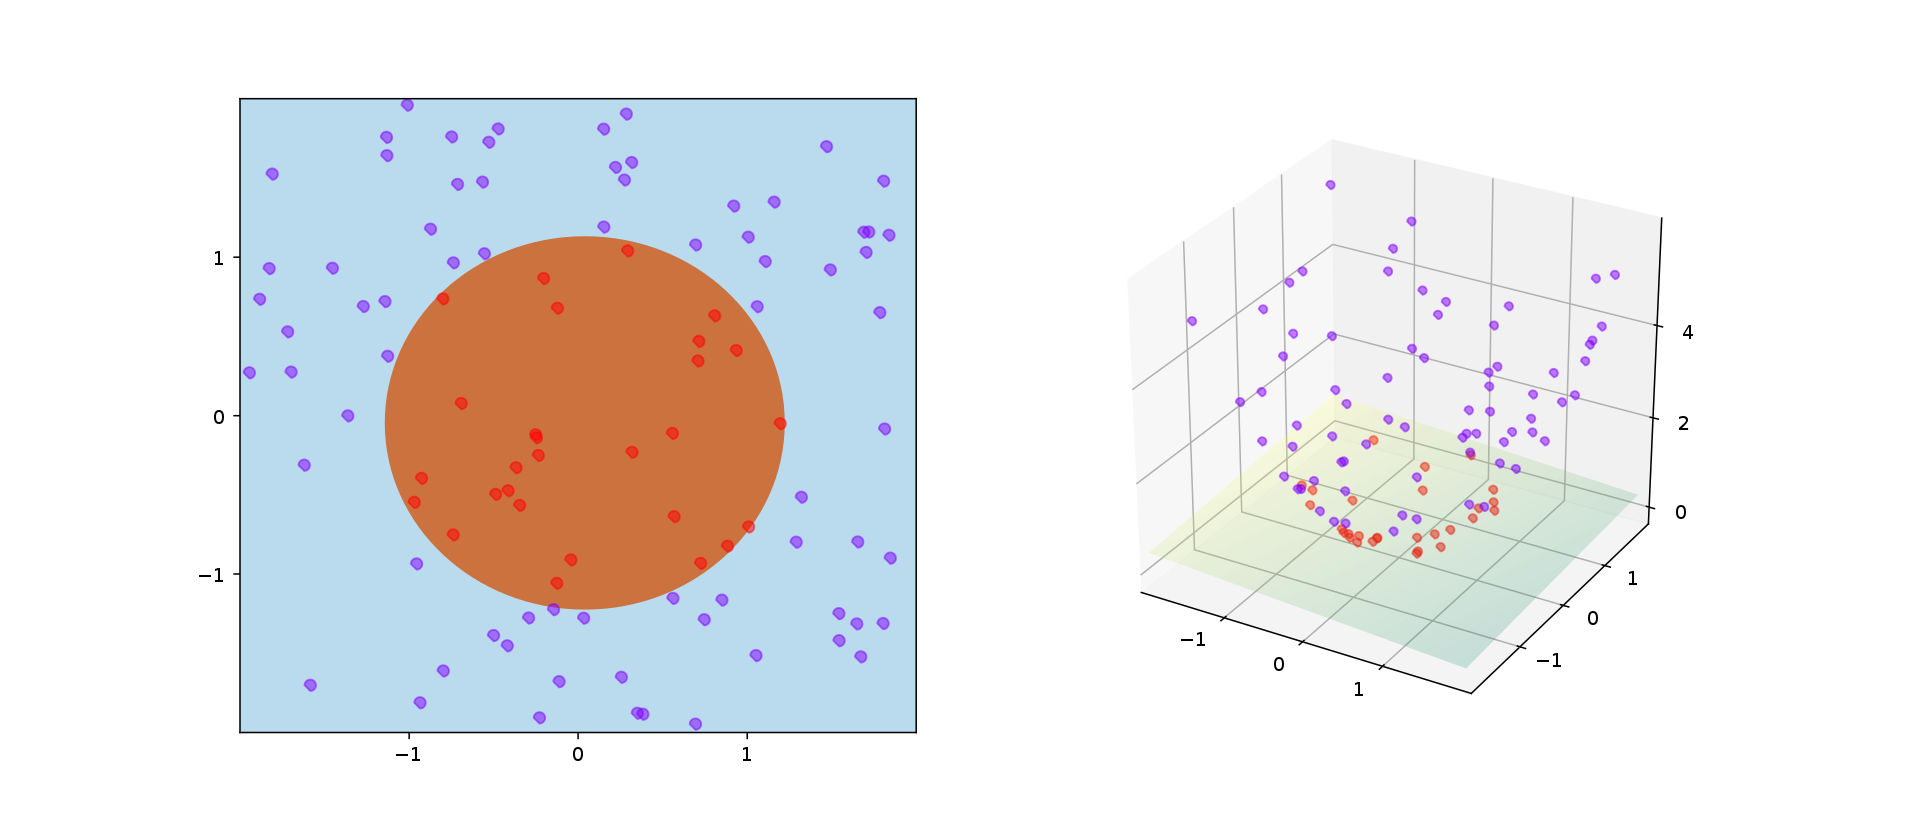
\includegraphics[width=10cm]{H1.png}
    \caption{Data linearly non-separable in 2D becomes linearly separable in 3D}
    \label{fig:Data linearlly non-separable in 2D becomes linearly separable in 3D}
    \end{figure}

    \subsection{Mercer's theorem}
Assume $\chi$ be an arbitrary non empty set of features. A function $k: \chi \times \chi \rightarrow \mathbb{R}$ is called a Mercer kernel function if there exists a Hilbert space $\mathcal{H}$ and a mapping $\phi$ which is defined as
$$
\begin{aligned}
&\phi: \chi \rightarrow \mathcal{H} \quad \text { s.t. } \forall x_{1}, x_{2} \in \chi \\
&k\left(x_{1}, x_{2}\right)=\left\langle\phi\left(x_{1}\right), \phi\left(x_{2}\right)\right\rangle_{\mathcal{H}}
\end{aligned}
$$
It can also be defined as a kernel function which satisfies the Mercer's condition.There exists a mapping $\Phi$ and an expansion $$
K(\mathbf{x}, \mathbf{y})=\sum_{i} \Phi(\mathbf{x})_{i} \Phi(\mathbf{y})_{i}
$$ for a kernel
if and only if, for all real valued functions $g(\mathbf{x})$ such that $\int g(\mathbf{x})^{2} d \mathbf{x}$ is finite then
$$
\int K(\mathbf{x}, \mathbf{y}) g(\mathbf{x}) g(\mathbf{y}) d \mathbf{x} d \mathbf{y} \geq 0 .
$$
The kernel functions should satisfy the above equation which is the Mercer's condition to be called a Mercer's kernel. If the kernel function satisfies Mercer's theorem then the dot product between two points in the Hilbert space can be replaced with the kernel function value between the same two points.
    
    \subsection{Popular kernels}
        \subsubsection{Linear kernels} Linear kernels are obtained by the dot product between the two vectors.
        $$
\kappa\left(\mathbf{x}, \mathbf{x}^{\prime}\right)=\mathbf{x}^{T} \mathbf{x}^{\prime}
$$
            and the corresponding mapping is $\phi(x)=x$.
        \subsubsection{Polynomial kernels} Polynomial kernel function is defined as 
        K$\left(\mathbf{x}^{(i)}, \mathbf{x}^{(j)}\right)=\left(\mathbf{x}^{(i)^{T}} \mathbf{x}^{(j)}+1\right)^{d}$ where d is the dimensionality of x.
        Quadratic kernels are used mostly in NLP problems where high dimensionality of RBF kernels might be a problem.
        
        \subsubsection{Gaussian kernels} A Gaussian kernel is defined as 
        $$\kappa\left(\mathbf{x}, \mathbf{x}^{\prime}\right)=\exp \left(-\frac{1}{2} \sum_{j=1}^{p} \frac{1}{\sigma_{j}^{2}} \cdot\left(x_{j}-x_{j}^{\prime}\right)^{2}\right)$$
        The dimensionality of the corresponding mapping $\Phi$ obtained is infinity.
        
    
\section{Primal vs Dual SVM}
The primal formulation of SVM in non-linear case is 
$$
\min \frac{1}{2} w^{T} w+C \sum_{i=1}^{l} \xi_{i}
$$
subject to
$$
\begin{aligned}
&y_{i}\left[w^{T} x_{i}+b\right] \geq 1-\xi_{i}, i=1, \ldots, l \\
&\xi_{i} \geq 0, i=1, \ldots, l .
\end{aligned}
$$
Here $\xi_{i}$'s are the slack variables, ($x_{i}$,$y_{i}$) are training data provided.
The KKT conditions for the above optimisation problem are 
\newline
- K1. $w-\sum_{i=1}^{l} \mu_{i} y_{i} x_{i}=0$.
\newline
- $\mathrm{K} 2 . \sum_{i=1}^{l} \mu_{i} y_{i}=0$.
\newline
- K3. $C-\mu_{i}-\lambda_{i}=0$.
\newline
- $\mathrm{K} 4.1-\xi_{i}-y_{i}\left(w^{T} x_{i}+b\right) \leq 0$.
\newline
- K5. $\xi_{i} \geq 0, \mu_{i} \geq 0, \lambda_{i} \geq 0, \forall i$.
\newline
- K6. $\mu_{i}\left[1-\xi_{i}-y_{i}\left(w^{T} x_{i}+b\right)\right]=0, \forall i$.
\newline
- K7. $\lambda_{i} \xi_{i}=0, \forall i$
\newline
The corresponding dual formulation of the problem is given by :
$$
\max \quad q(\mu)=\sum_{i=1}^{l} \mu_{i}-\frac{1}{2} \sum_{i, j=1}^{l} \mu_{i} \mu_{j} y_{i} y_{j} x_{i}^{T} x_{j}
$$
subject to
$$
\begin{aligned}
&0 \leq \mu_{i} \leq C, \forall i \\
&\sum_{i=1}^{l} \mu_{i} y_{i}=0
\end{aligned}
$$
The solution of the primal is an upper bound on the solution of dual and solution of dual is lower bound on the solution of primal.For a convex optimisation problem both the solutions become same which is the optimal solution.

\section{Kernel SVM}
For non-linear case we may not get good results with the non-linear optimisation problem in the above section. Another approach is to use nonlinear SVM's which uses kernel idea to project the data to a high dimensional space without actually knowing the mapping or the space. The optimisation problem for the nonlinear SVM case is given by 
$$
\max  q(\mu)=\sum_{i=1}^{l} \mu_{i}-\frac{1}{2} \sum_{i, j=1}^{l} \mu_{i} \mu_{j} y_{i} y_{j} K\left(x_{i}, x_{j}\right) \\
\text { subject to }  0 \leq \mu_{i} \leq C, \quad i=1, \ldots, l \\
 \sum_{i=1}^{l} \mu_{i} y_{i}=0
$$

The value of b and W is obtained by 
$$
f(x)=\sum_{i \in S} \mu_{i} y_{i} K\left(x_{i}, x\right)+b .
$$
Here, $S=\left\{i: \mu_{i}>0\right\}$ and $b$ is given by
$$
b=y_{j}-\sum_{i \in S} \mu_{i} y_{i} K\left(x_{i}, x_{j}\right)
$$
The above optimisation problem is Quadratic Optimisation problem (QP) with one equality and one inequality constraints.

\section{PCA vs Kernel PCA}
    \subsection{PCA}
We assume that the data we have is mean centered i.e. given observations $\mathbf{x}_{k}, k=1, \ldots, M, \mathbf{x}_{k} \in \mathbf{R}^{N}, \sum_{k=1}^{M} \mathbf{x}_{k}=0$. PCA tries to diagonalise the covariance matrix given by $C=\frac{1}{M} \sum_{j=1}^{M} \mathbf{x}_{j} \mathbf{x}_{j}^{\top}$ by solving the eigen value problem $\lambda \mathbf{v}=C \mathbf{v}$.
Then we get the projections of the data on these eigen vectors to get the new samples.The main disadvantage of PCA is that we may loose some cluster properties and neighbourhood infformation since PCA is basically a linear transform. To deal with this drawback one can make use of kernel PCA which is discussed below.
    \subsection{Kernel PCA}
In kernel PCA, we first project the data to a very high dimension so that it becomes linear in the high dimension and then we transform the data to a lower dimension using a linear transform. 
/newline
Emperical co-variance operator is given by.
$$
\hat{\Sigma}=\frac{1}{n} \sum_{i=1}^{n} \phi\left(x^{i}\right) \otimes \phi\left(x^{i}\right)
$$
We want to get direction where variance is maximised in the new space. i.e like in PCA we want to solve eigen value problem in the high dimensional space.
$$
(\hat{\Sigma})(\hat{\phi})=\lambda(\hat{\phi})
$$
We can assume $$\hat{\phi}=\sum_{i=1}^{n} \alpha_{i} \phi\left(x^{i}\right)$$ where $\alpha_{i} \in R$. 
This is valid because consider $\hat{\phi}=\hat{\phi}^{\perp}+\hat{\phi}^{in}$ where
$\hat{\phi}^{in}$= component of $\hat{\phi}$ is in span of $\phi\left(x^{i}\right)$ and
$\hat{\phi}^{\perp}$= component of $\hat{\phi}$ perpendicular to the span of $\phi\left(x^{\prime}\right)$. $\hat{\phi}^{\perp} \cdot \phi\left(x^{i}\right)=0 \quad \forall i=1 . n$. Hence it is a valid assumption.
Multiplying by $\hat{\phi}$
$$
\hat{\Sigma}(\hat{\phi})=\frac{1}{n} \sum_{i=1}^{n}\left\langle\phi\left(x^{i}\right), \hat{\phi}\right\rangle \phi\left(x^{i}\right) \text {. }
$$
The eigen vector equation becomes
$$
\hat{\Sigma}\left(\sum_{i=1}^{n} \alpha_{i} \phi\left(x^{i}\right)\right)=\lambda \sum_{i=1}^{n} \alpha_{i} \phi\left(x^{i}\right)
$$
From above we have,
$$
\text { LHS }=\frac{1}{n} \sum_{i=1}^{n} \sum_{j=1}^{n} \alpha_{i}\left\langle\phi\left(x^{i}\right), \phi\left(x^{j}\right)\right\rangle \phi\left(x^{j}\right)
$$
But $k\left(x^{i}, x^{j}\right)=\left\langle\phi\left(x^{i}\right), \phi\left(x^{j}\right)\right\rangle$
so the equation becomes
$$
\frac{1}{n} \sum_{i, j=1}^{n} \alpha_{i} k\left(x^{i}, x^{J}\right) \phi\left(x^{\mathrm{j}}\right)=\lambda \sum_{i=1}^{n} \alpha_{i} \phi\left(x^{i}\right)
$$
taking inner product with $\phi\left(x^{l}\right) \quad l=1,2 \ldots n$
$$
\frac{1}{n} \sum_{i, j=1}^{n} \alpha_{i} k\left(x^{i}, x^{J}\right) k\left(x^{j}, x^{\ell}\right)=\lambda \sum_{i=1}^{n} \alpha_{i} k\left(x^{i}, x^{\ell}\right)
$$
In matrix form
$$
K^{2} \alpha=\lambda_{n} K \alpha \quad K \in R^{n \times n} .
$$
so $$K \alpha=\lambda n \alpha$$.
which is similar to the eigen value problem in normal PCA but here instead of the covariance matrix use the Kernal matrix K.

\subsubsection{Examples showing the effectiveness of Kernel PCA}
The code for the examples and figures are available at:
    \begin{figure}[htp]
    \centering
    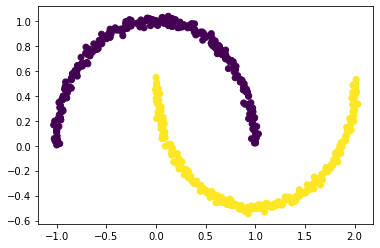
\includegraphics[width=10cm]{H2.png}
    \caption{Original 2D data}
    \label{Original 2D data}
    \end{figure}
    \begin{figure}[htp]
    \centering
    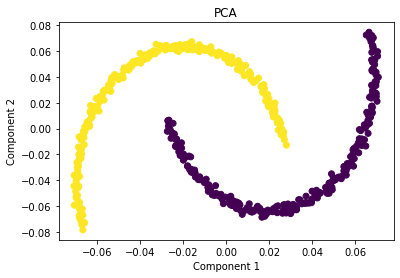
\includegraphics[width=10cm]{H3.png}
    \caption{Data after doing normal PCA in 2D}
    \label{Data after doing normal PCA in 2D}
    \end{figure}
\begin{figure}[htp]
    \centering
    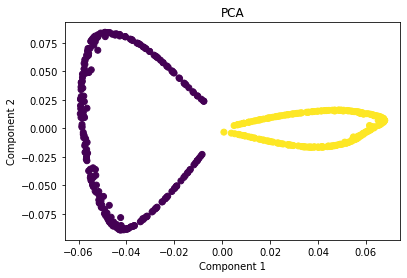
\includegraphics[width=10cm]{H4.png}
    \caption{Data after doing Kernel PCA in 2D}
    \label{Data after doing Kernel PCA in 2D}
    \end{figure}


\section{Kernel optimisation}
Till now in all the algorithms the kernels were fixed i.e. we chose kernels depending on our intuitions. This section deals with learning the data-dependent kernel along with the optimisation problem.Let us see one of the methods of optimising kernel.For this we define the following class separability measure $$J=\frac{\operatorname{tr} S_{b}}{\operatorname{tr} S_{w}}$$ 
where 
$$
\begin{aligned}
S_{b} &=\frac{1}{m} \sum_{i=1}^{2} m_{i}\left(\bar{y}_{i}-\bar{y}\right)\left(\bar{y}_{i}-\bar{y}\right)^{T} \\
S_{w} &=\frac{1}{m} \sum_{i=1}^{2} \sum_{j=1}^{m_{i}}\left(y_{j}^{i}-\bar{y}_{i}\right)\left(y_{j}^{i}-\bar{y}_{i}\right)^{T}
\end{aligned}
$$
$S_{b}$ is called the Between-class cluster and $S_{w}$ is called within class cluster.We can derive the kernel formulation of class separability measure and solve the optimisation problem. Since the algorithm or technique was covered in detail in another lecture we are going to skip the details in this notes.

\section{SVM regression non-linear case}
We will now discuss how to use the SVM for solving the regression problem. Here we will discuss $\epsilon$ tube regression idea where the loss function is defined as  

$$L(y, g(x, w, b)) =0 \quad \text { if }|y-g(x, w, b)|<\epsilon$$
$$L(y, g(x, w, b)) =|y-g(x, w, b)|-\epsilon \quad \text { otherwise. }
$$
The primal optimisation problem for the above loss function is given by 
$$
\min \quad  \frac{1}{2} w^{T} w+C \sum_{i=1}^{l}\left(\xi_{i}+\xi_{i}^{\prime}\right)$$
$$
\text { subject to }  y_{i}-w^{T} \phi\left(x_{i}\right)-b \leq \epsilon+\xi_{i}, i=1, \ldots, l$$
$$ w^{T} \phi\left(x_{i}\right)+b-y_{i} \leq \epsilon+\xi_{i}^{\prime}, i=1, \ldots, l$$
$$ \xi_{i} \geq 0, i=1, \ldots, l $$
$$ \xi_{i}^{\prime} \geq 0, i=1, \ldots, l
$$

The linear case is simpler and the optimisation problem is exactly equal to the above optimisation problem without the slack variables ($ \xi_{i}$). The corresponding dual of the problem can be solved and the dual optimisation problem is given by 
$$
\begin{aligned}
\max & \sum_{i=1}^{l} y_{i}\left(\mu_{i}-\mu_{i}^{\prime}\right)-\epsilon \sum_{i=1}^{l}\left(\mu_{i}+\mu_{i}^{\prime}\right)-\frac{1}{2} \sum_{i, j=1}^{l}\left(\mu_{i}-\mu_{i}^{\prime}\right)\left(\mu_{j}-\mu_{j}^{\prime}\right) \phi\left(x_{i}\right)^{T} \phi\left(x_{j}\right) \\
\text { subject to } \quad & 0 \leq \mu_{i}, \mu_{i}^{\prime} \leq C, \forall i \\
& \sum_{i=1}^{l}\left(\mu_{i}-\mu_{i}^{\prime}\right)=0
\end{aligned}
$$
Although we get good results for the regression using the above optimisation technique there is a big problem at the heart of the primal equation. There is no physical significance for W in the above optimisation problem while in classification formulation minimising W leads to higher margin. Here there is no physical meaning for minimising W other than the notion of considering it as a regularisation term. We will discuss more about the significance of W in the section Regression to Classification.

\subsection{Non-linear SVM regression using Kernels}
We can extend the above idea of regression to use kernel methods which will ensure more linearity at higher dimensions according to the Cover's theorem.The optimisation problem is very closely related to the dual formulation for regression with the exception of dot product being replaced by a positive semi-definite kernel matrix K.

$$
\max \sum_{i=1}^{l} y_{i}\left(\mu_{i}-\mu_{i}^{\prime}\right)-\varepsilon \sum_{i=1}^{l}\left(\mu_{i}+\mu_{i}^{\prime}\right)-\frac{1}{2} \sum_{i, j=1}^{\ell}\left(\mu_{i}-\mu_{i}^{\prime}\right)\left(\mu_{j}-\mu_{j}^{\prime}\right) K\left(x^{i}, x j\right)$$
$$\text { subject to } \quad  0 \leqslant \mu_{i}, \mu_{i}^{\prime} \leq C $$
$$\sum_{i=1}^{l}\left(\mu_{i}-\mu_{i}^{\prime}\right)=0 .
$$


\section{Regression to classification}
As already mentioned one problem with the regression formulation of SVM is that there is no physical significance for minimising W.Another very important limitation is that there is no notion of model complexity or VC dimension in case of SVR(Support Vector Regression). In this section we will see how Bi and Bennett tried to convert the regression problem to a classification problem so that all notions and ideas like VC dimension,etc can be applied to a regression problem as well.
\newline
The basic idea is that we create two classes for +1 class and for -1 class. Once we have the two classes we can apply all the SVM algorithms developed for classification problem including dual and kernel formulations.
$$D^{+}=\left\{\left(\begin{array}{l}
x_{i} \\
y_{i}+\varepsilon
\end{array}\right), i=1, \ldots l\right\} .$$
$$D^{-}=\left\{\left(\begin{array}{l}
x_{i} \\
y_{i}-\varepsilon
\end{array}\right), i=1, \ldots l\right\} .$$
    \begin{figure}[htp]
    \centering
    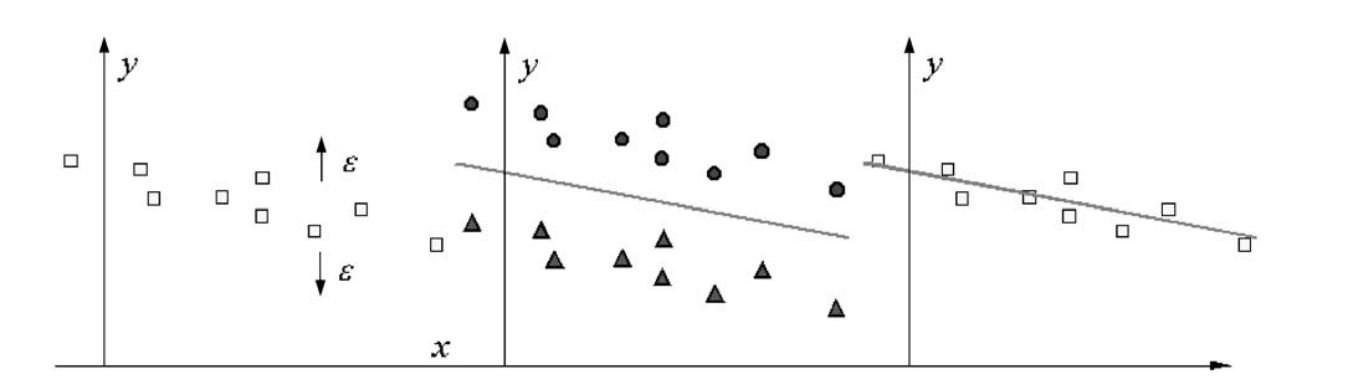
\includegraphics[width=10cm]{H5.png}
    \caption{Conversion from regression to classification}
    \label{Conversion from regression to classification}
    \end{figure}
\section{Experiments and Implementations}
In this section we will showcase the results of implementing the above algorithms in python. The code and results will be available in github at :

\subsection{DUAL VS PRIMAL SVM}
The optimisation codes for primal and dual SVM's were written and results compared. 
    \begin{figure}[htp]
    \centering
    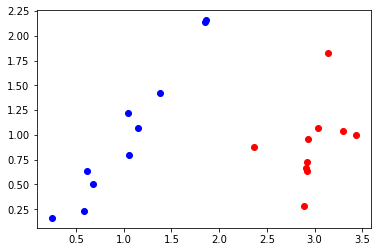
\includegraphics[width=10cm]{H6.png}
    \caption{Data used for training SVM}
    \label{Data used for training SVM}
    \end{figure}
\subsubsection{Primal SVM results}
Weights obtained for the above data: -1.59871784,  1.17456189
Bias obtained:1.74919393
    
\subsubsection{Dual SVM results}
Weights obtained for the above data: -1.58388965,  0.94189243
Bias obtained:1.91898122
Number of support vectors=3
\newline 
As one can observe the weights obtained from primal and dual does not exactly match but they are within an error range.

    \begin{figure}[htp]
    \centering
    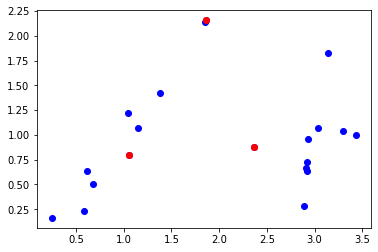
\includegraphics[width=10cm]{H7.png}
    \caption{Red dots are the support vectors for the data in figure 1.6}
    \label{Red dots are the support vectors for the data in figure 1.6}
    \end{figure}


\subsection{Kernel SVM}
This subsection deals with results obtained with the kernel implementation of the SVM.We will try to compare the results obtained when data is non-linearly separable in original dimension.

    \begin{figure}[htp]
    \centering
    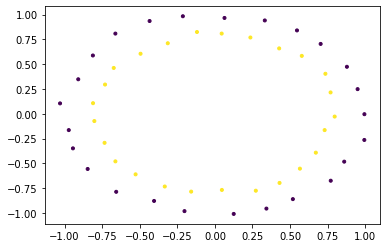
\includegraphics[width=10cm]{H12.png}
    \caption{Original Data}
    \label{Original Data}
    \end{figure}

Kernel SVM accuracy score on training data: 0.52
\newline
Linear SVM accuracy score on training data: 0.50
\newline
As we can clearly see kernel SVM performs better on non-linear data as it will project the data to a very high dimension where the data will be linearly separable. Note that there is no significant increase because the optimisation code for kernel SVM is not optimised

\subsection{Kernel PCA}
We will now look at how kernel methods can enhance dimensionality reduction techniques like PCA.
\newline
From Figure 1.7 and 1.8 it is very clear that normal PCA is unable to infer information about the labels or geometric structure of the data whereas kernel PCA(Guaussian kernel) was able to preserve the geometric information of the data.
    


    \begin{figure}[htp]
    \centering
    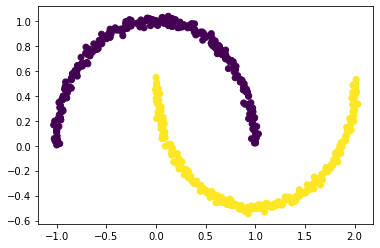
\includegraphics[width=9cm]{H10.png}
    \caption{Original Data}
    \label{Original Data}
    \end{figure}
    
    \begin{figure}[htp]
    \centering
    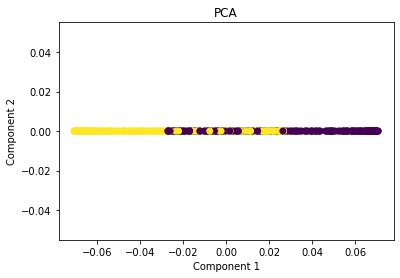
\includegraphics[width=10cm]{H8.png}
    \caption{Normal PCA in 1D}
    \label{Normal PCA in 1D}
    \end{figure}
    
    \begin{figure}[htp]
    \centering
    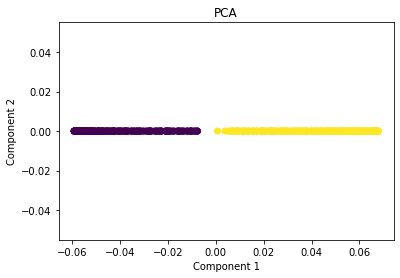
\includegraphics[width=9cm]{H9.png}
    \caption{Kernel PCA in 1D}
    \label{Kernel PCA in 1D}

    \end{figure}

Figure 1.9 shows the distribution of original data. When we apply normal PCA on this we get an overlapped region on as we can see in Figure 1.10. But Figure 1.11 shows that this problem does not exist in kernel PCA as data is well separated for the two classes.
\newline
\newline
\newline

\subsection{SVM Regression}
In this section we will compare the results from normal SVM regression and regression using Gaussian kernel.
\subsubsection{Non linear case}

    \begin{figure}[htp]
    \centering
    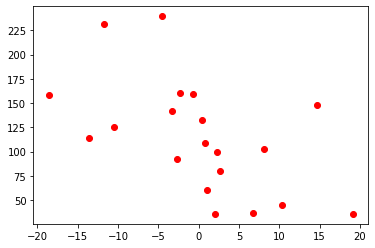
\includegraphics[width=10cm]{H13.png}
    \caption{Non linear data}
    \label{Non linear data}
    \end{figure}
r2 score obtained for non-linear data with kernel SVM:0.9999933197143883. As it is clear from the r2-score we were able to get good fit even on the non linear data.



\subsection{Regression to classification}
In this section we will see the implementation of Bi and Bennett of converting regression to classification and then using SVM classifier to get the weights of the line.
\newline
The basic idea is that we create two classes for +1 class and for -1 class. Once we have the two classes we can apply all the SVM algorithms developed for classification problem including dual and kernel formulations.
$$D^{+}=\left\{\left(\begin{array}{l}
x_{i} \\
y_{i}+\varepsilon
\end{array}\right), i=1, \ldots l\right\} .$$
$$D^{-}=\left\{\left(\begin{array}{l}
x_{i} \\
y_{i}-\varepsilon
\end{array}\right), i=1, \ldots l\right\} .$$
Original equation of the line from which data is sampled Y = 6x1+5x2. We make two datasets for +1 class and -1 class. Theory is discussed in detail in section 1.8.
The equation obtained by solving the classification problem using SVM is 
6.00*x1+5.00*x2. As one can observe we got the same equation of the regression line.
    
    \begin{figure}[htp]
    \centering
    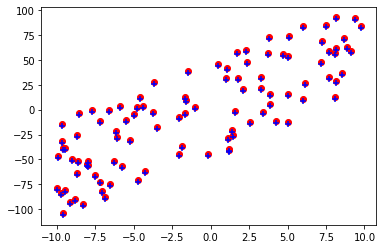
\includegraphics[width=10cm]{H11.png}
    \caption{Classification problem for the regression problem Y=6x1+5x2.Dots are -1 class and + is +1 class}
    \label{Classification problem for the regression problem Y=6x1+5x2}
    \end{figure}

    
    
	\bibliographystyle{plain}
	\begin{thebibliography}{10}
		\bibitem{mr:random}
	A geometric approachto support vector
regression Jinbo Bi , Kristin P. Bennett 
	\bibitem{mr:random}
	An Introduction to Support Vector Machines
P. S. Sastry
	\bibitem{mr:random}
	Nonlinear Component Analysis as a Kernel Eigenvalue
Problem
Bernhard Sch¨olkopf
Alexander Smola
Klaus-Robert M ¨uller
	\bibitem{mr:random}
Optimizing the Kernel in the Empirical Feature Space
Huilin Xiong, M. N. S. Swamy, Fellow, IEEE, and M. Omair Ahmad, Fellow, IEEE
		\bibitem{mr:random}
Wikipedia

	\end{thebibliography}

\end{document}